% Copyright (c) 2022 by Lars Spreng
% This work is licensed under the Creative Commons Attribution 4.0 International License. 
% To view a copy of this license, visit http://creativecommons.org/licenses/by/4.0/ or send a letter to Creative Commons, PO Box 1866, Mountain View, CA 94042, USA.

%~~~~~~~~~~~~~~~~~~~~~~~~~~~~~~~~~~~~~~~~~~~~~~~~~~~~~~~~~~~~~~~~~~~~~~~~~~~~~~
% You can add your packages and commands to the loadslides.tex file. 
% The files in the folder "styles" can be modified to change the layout and design of your slides.
% I have included examples on how to use the template below. 
% Some of it these examples are taken from the Metropolis template.
%~~~~~~~~~~~~~~~~~~~~~~~~~~~~~~~~~~~~~~~~~~~~~~~~~~~~~~~~~~~~~~~~~~~~~~~~~~~~~~

\documentclass[
11pt,notheorems,hyperref={pdfauthor=whatever}
]{beamer}


% Copyright (c) 2022 by Lars Spreng
% This work is licensed under the Creative Commons Attribution 4.0 International License. 
% To view a copy of this license, visit http://creativecommons.org/licenses/by/4.0/ or send a letter to Creative Commons, PO Box 1866, Mountain View, CA 94042, USA.

%~~~~~~~~~~~~~~~~~~~~~~~~~~~~~~~~~~~~~~~~~~~~~~~~~~~~~~~~~~~~~~~~~~~~~~~~~~~~~~
% Add your packages and commands to this file
%~~~~~~~~~~~~~~~~~~~~~~~~~~~~~~~~~~~~~~~~~~~~~~~~~~~~~~~~~~~~~~~~~~~~~~~~~~~~~~

%~~~~~~~~~~~~~~~~~~~~~~~~~~~~~~~~~~~~~~~~~~~~~~~~~~~~~~~~~~~~~~~~~~~~~~~~~~~~~~
\RequirePackage{palatino}
\RequirePackage[utf8]{inputenc}
\RequirePackage[T1]{fontenc}

\usefonttheme{serif}

\usepackage{styles/elegantmacros}
\usefolder{styles}
\usetheme[style=blue]{elegant}

\newcommand{\makepart}[1]{ % For convenience
\part{#1} \frame{\partpage}
} 

%~~~~~~~~~~~~~~~~~~~~~~~~~~~~~~~~~~~~~~~~~~~~~~~~~~~~~~~~~~~~~~~~~~~~~~~~~~~~~~

%~~~~~~~~~~~~~~~~~~~~~~~~~~~~~~~~~~~~~~~~~~~~~~~~~~~~~~~~~~~~~~~~~~~~~~~~~~~~~~
% Figures
\RequirePackage{booktabs}
\RequirePackage{colortbl}
\RequirePackage{ragged2e}
\RequirePackage{schemabloc}
%\RequirePackage{natbib}
\RequirePackage{caption}
\RequirePackage{subcaption}
\RequirePackage{tabularx}
\RequirePackage{array}
\RequirePackage{multirow}
\usepackage[
  style=authoryear, 
]{biblatex}
\RequirePackage{xcolor}
\addbibresource{references.bib}
\newcolumntype{Y}{>{\centering\arraybackslash}X}

%~~~~~~~~~~~~~~~~~~~~~~~~~~~~~~~~~~~~~~~~~~~~~~~~~~~~~~~~~~~~~~~~~~~~~~~~~~~~~~

%~~~~~~~~~~~~~~~~~~~~~~~~~~~~~~~~~~~~~~~~~~~~~~~~~~~~~~~~~~~~~~~~~~~~~~~~~~~~~~
% Figures
\RequirePackage{wrapfig}
\RequirePackage{pgfplots}
\RequirePackage{graphicx}
\RequirePackage{adjustbox}
\RequirePackage{environ}
\pgfplotsset{compat=1.18  }

\makeatletter
\newsavebox{\measure@tikzpicture}
\NewEnviron{scaletikzpicturetowidth}[1]{%
  \def\tikz@width{#1}%
  \def\tikzscale{1}\begin{lrbox}{\measure@tikzpicture}%
  \BODY
  \end{lrbox}%
  \pgfmathparse{#1/\wd\measure@tikzpicture}%
  \edef\tikzscale{\pgfmathresult}%
  \BODY
}
\makeatother
%~~~~~~~~~~~~~~~~~~~~~~~~~~~~~~~~~~~~~~~~~~~~~~~~~~~~~~~~~~~~~~~~~~~~~~~~~~~~~~

%~~~~~~~~~~~~~~~~~~~~~~~~~~~~~~~~~~~~~~~~~~~~~~~~~~~~~~~~~~~~~~~~~~~~~~~~~~~~~~
% Maths 
\RequirePackage{textcomp}
\RequirePackage{amsmath} 
\RequirePackage{amsthm}
\RequirePackage{mathtools}
\RequirePackage{braket}
%\RequirePackage{bbm}
%\RequirePackage{algorithm}
%\RequirePackage[osf,sc]{mathpazo}
%\RequirePackage{pifont}
%\newcommand{\xmark}{\ding{55}}%
%\numberwithin{equation}{section}
\DeclareMathOperator*{\argmax}{arg\,max}
\DeclareMathOperator*{\argmin}{arg\,min}

\setbeamertemplate{theorems}[numbered] % to number

\theoremstyle{definition}
\newtheorem{fact}{Fact}[section]
\newtheorem{examp}{Example}[section]

\theoremstyle{plain}
\newtheorem{definition}{Definition}[section]
\newtheorem{proposition}{Proposition}
\newtheorem{theorem}{Theorem}
\newtheorem{assumption}{Assumption}

\providecommand{\H}{\mathscr{H}}      
\providecommand{\E}{\mathbb{E}}
\makeatletter
\def\munderbar#1{\underline{\sbox\tw@{$#1$}\dp\tw@\z@\box\tw@}}
\makeatother

%~~~~~~~~~~~~~~~~~~~~~~~~~~~~~~~~~~~~~~~~~~~~~~~~~~~~~~~~~~~~~~~~~~~~~~~~~~~~~~
%Commands
\newcommand{\importanttext}[1]{\Large #1 \normalsize}
\newcommand{\crt}[1]{a_{#1}^{\dagger}}
\newcommand{\ani}[1]{a_{#1}}
\newcommand{\vac}{\ket{0}}
\newcommand{\gs}{\ket{\Phi_0}}
\newcommand{\exed}[2]{\ket{\Phi_{#1}^{#2}}}

\newcommand{\inner}[3]{\bra{#1}#2\ket{#3}}
\newcommand{\innerAS}[3]{\inner{#1}{#2}{#3}_{\text{AS}}}
\newcommand{\mathset}[1]{\{ #1 \}}
\newcommand{\ord}[2]{#1^{(#2)}}
\newcommand{\energyref}{E_0^{\text{ref}}}
\newcommand{\psum}{\sideset{}{'}\sum}

\newcommand{\spinop}[1]{\hat{S}_{#1}}
\newcommand{\pplus}[1]{\hat{P}_{#1}^{+}}
\newcommand{\pminus}[1]{\hat{P}_{#1}^{-}}
\newcommand{\numberop}[1]{\hat{N}_{#1}}
\newcommand{\hatreefock}[1]{#1^{\text{HF}}}
\newcommand{\comment}[1]{\textcolor{red}{#1}}
\newcommand{\functional}[1]{\[ #1 \}}

% Colors
\definecolor{Green}{RGB}{20, 128, 10}
\definecolor{Red}{RGB}{153, 22, 8} % Loads packages and some defined commands

\title[
% Text entered here will appear in the bottom middle
]{FYS4480 Oral exam, midterm one and two}

\subtitle{Helium and Beryllium using CIS and Hartree-Fock, pairing model}

\author[
% Text entered here will appear in the bottom left corner
]{
    Håkon Kvernmoen
}

\institute{
    University of Oslo}
\date{\today}

\begin{document}

% Generate title page
{
\setbeamertemplate{footline}{} 
\begin{frame}
  \titlepage
\end{frame}
}
\addtocounter{framenumber}{-1}

% You can declare different parts as a parentof sections
% \begin{frame}{Part I: Demo Presentation Part}
%     \tableofcontents[part=1]
% \end{frame}
% \begin{frame}{Part II: Demo Presentation Part 2}
%     \tableofcontents[part=2]
% \end{frame}

% \makepart{Demo Part}

% \section{Introduction}
% \begin{frame}
% \begin{itemize}
%     \item This template provides an elegant and minimalistic layout for beamer slides. Hence the name \alert{\textbf{Elegant Slides}}.
%     \item I created Elegant Slides because I wasn't satisfied with any of the existing Beamer templates, which look slightly different than Elegant Slides.
%     \item My goal was to create a layout that is \alert{\textbf{simplistic but beautiful}} and focuses on the content, rather than crowding each slide with lots of different coloured boxes.
%     \item I designed Elegant Slides for \alert{\textbf{lecture notes and technical presentations}} but it can be used for any kind of talk. 
% \end{itemize}
     
% \end{frame}

\begin{frame}
    \frametitle{Setup}
    Represent states using creation $\crt{p}$ and annihilation $\ani{q}$ operators (occupation representation/second quantization), obeying
    \begin{align*}
        \mathset{\crt{p},\ani{q}} = \delta_{pq},\hspace{20px}\mathset{\crt{p},\crt{q}} = \mathset{\ani{p},\ani{q}} = 0
    \end{align*}
    $p$ and $q$ are sets of relevant quantum numbers. We need to pick a single particle (SP) computational basis, having $n$ possible single particle states.
    \begin{align*}
        \text{3D HO:}\hspace{20px}p = \mathset{n_r,l,m_l,s,m_s},\hspace{20px} \crt{p} \vac = \ket{p} \longrightarrow \psi_p(\bold{x}) = \psi_{n_r l m}(r, \theta, \phi) = \ldots 
    \end{align*} 
    Need a Hamiltonian to solve $\hat{H} = \hat{H}_0 + \hat{V}$, with $\hat{H}_0$ representing single particle energy contributions, and $\hat{V}$ interactions.
    \\[10pt]
    Often start with an $N$-particle ground state ansatz $\ket{\Phi_0} = \crt{1},\ldots \crt{N} \vac$.
    \\[10pt]
    And consider excitations of this
    \begin{align*}
        \text{1p1h}\hspace{20px}&\exed{i}{a} = \crt{a}\ani{i}\gs \\
        \text{2p2h}\hspace{20px}&\exed{ij}{ab} = \crt{a}\crt{b}\ani{j}\ani{i}\gs  \\
        \text{NpNh}\hspace{20px}&\exed{ij\ldots}{ab\ldots} = \crt{a}\crt{b}\ldots\ani{j}\ani{i}\gs 
    \end{align*}
\end{frame}


\subsection{FCI}
\begin{frame}
    \frametitle{Full configuration interaction (FCI)}

    Start with $N$ particle ground state ansatz $\ket{\Phi_0}$.
    \\[10pt]
    Not an eigenstate of $\hat{V}$ and therefor not the true ground state of the system.
    \\[10pt]
    By considering every possible $N$ particle state in our system (using $\mathset{\crt{1},\ldots,\crt{N},\ldots,\crt{n}}$), we can construct our ground state $\ket{\Psi_0}$ as a linear combination of excited states.
    \begin{align*}
        \ket{\Psi_0} = C_0\gs + \sum_{ai} C_i^a \exed{i}{a} + \sum_{abij} C_{ij}^{ab} \exed{ij}{ab} + \ldots
    \end{align*} 
    \\[10pt] 
    Normally solved by considering the Hamiltonian in matrix representation, with elements $H_{XY} = \inner{\Phi_X}{\hat{H}}{\Phi_Y}$, with $X, Y \in \mathset{\text{0p0h},\text{1p1h}\ldots\text{NpNh}}$, giving the eigenvalue problem 
    \begin{align*}
        H \bold{c} = E\bold{c}
    \end{align*}
    When solved, the smallest eigenvalue $\ord{E}{0}$ will yield the ground state energy, and $\ket{\Psi_0}$ can be found by considering the eigenvectors $\ord{\bold{c}}{0} = (C_0, C_{i}^{a} \ldots C_{ij}^{ab} \ldots \ldots C_{ij\ldots}^{ab\ldots})$. Excited states can also be found by considering the other eigenvalues and vectors $\ord{E}{i}, \ord{\bold{c}}{i}$.
\end{frame}

\subsection{FCI}
\begin{frame}
    Example, pairing interaction: $\hat{V}$ only works between spin-paired states at the same energy level. We let $p = 1, 2, 3, 4$ denote energy levels, with SP states also having a spin $\sigma = \pm$, a total of $n = 8$ SP states. 
    \begin{align*}
        \hat{H} = \hat{H}_0 + \hat{V},\hspace{20px} \hat{H}_0 = \sum_{p\sigma} (p-1)\crt{p\sigma}\ani{p\sigma}, \hspace{20px}\hat{V} = -\frac{1}{2}g\sum_{pq}\crt{p+}\crt{p-}\ani{q-}\ani{q+}
    \end{align*}
    Diagonal SP Hamiltonian $\hat{H}_0$ and two body interaction $\hat{V}$. Consider $N = 4$ particles with total spin $S = 0$, writing $\ket{PQ} = \ket{p+p-q+q-}$ we have a total of six different many body states.
    \begin{align*}
        \text{0p0h}&\hspace{20px} \ket{12}  \\
        \text{2p2h}&\hspace{20px} \ket{13}, \ket{14}, \ket{23}, \ket{24} \\  
        \text{4p4h}&\hspace{20px} \ket{34}
    \end{align*}
    By setting up the matrix $\inner{KL}{\hat{H}}{RS}$, we get a small eigenvalue problem of a $6 \times 6$ matrix.
\end{frame}

\subsection{FCI}
\begin{frame}
    \begin{figure}
        \centering
        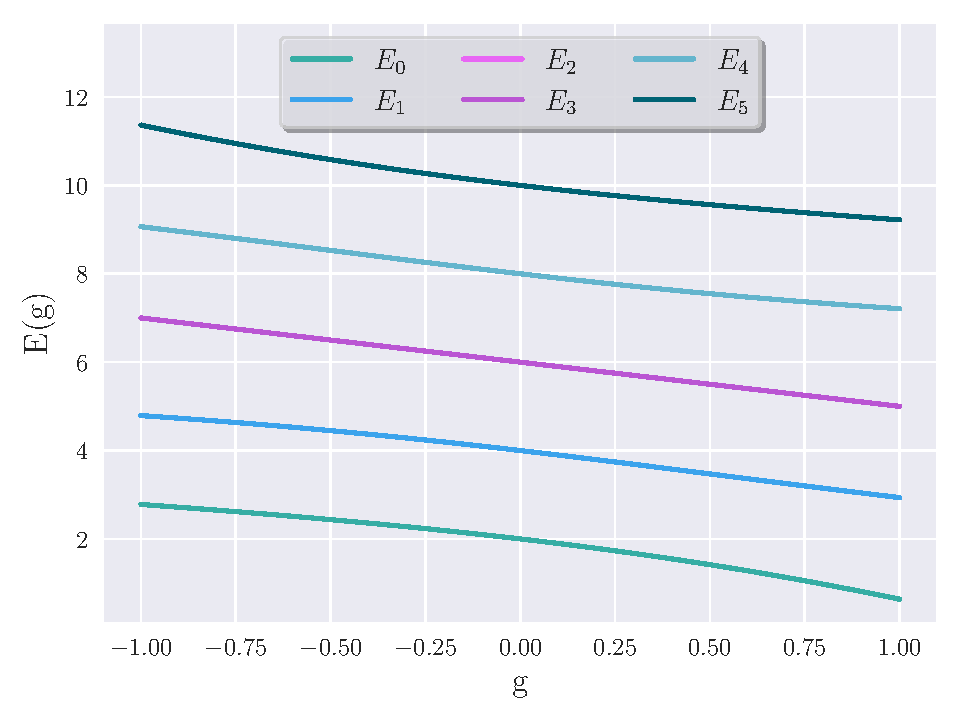
\includegraphics[width=0.75\linewidth]{figs/FCI.pdf}
    \end{figure}
    But there is a problem...
\end{frame}

\subsection{FCI}
\begin{frame}
    For all but very simple problems, this approach is unfeasible. In general, we have to consider 
    \begin{align*}
        \binom{n}{N} = \frac{n!}{N!(n-N)!}
    \end{align*}
    many body states. Taking our pairing model example, lifting the $S = 0$ restriction yields 70 different states. This is still possible, but increasing both $n$ and $N$ results in disaster
    
    \begin{table}
        \begin{tabular}{c|l|l|l|l}
        $N \downarrow /n \rightarrow$ & 8    & 32       & 64        & 128       \\
        \hline
        4     & $70$ & $10^{4}$ & $10^{5}$  & $10^{7}$  \\
        8     &      & $10^{7}$ & $10^{9}$  & $10^{12}$ \\
        16    &      & $10^{8}$ & $10^{14}$ & $10^{19}$ \\
        32    &      &          & $10^{18}$ & $10^{30}$
        \end{tabular}
        \caption{NB: Order of magnitude values}
    \end{table}
\end{frame}

\subsection{FCI}
\begin{frame}
    \textcolor{Green}{\importanttext{Pros:}}
    \begin{itemize}
        \item Provides exact solutions within a truncated basis set
        \item Understandable and relatively easy to set up 
        \item Excited states thrown into the bargain
    \end{itemize}
    \vspace{20px}
    \textcolor{Red}{\importanttext{Cons:}}
    \begin{itemize}
        \item Computational complexity, bad scaling
        \item Only possible for tiny systems, with few states and particles.
        \item Practically only a benchmarking tool
    \end{itemize}
\end{frame}

\begin{frame}
    \frametitle{Configuration Interaction (CI)}
    Follows the same methodology as FCI, but due to its large computational time, the many body states are also truncated.
    \\[10pt]
    Different truncation levels can be chosen, for instance only include (in addition to $\gs$) 1p1h excitations (CIS) or 2p2h excitations (CID).
    \\[10pt]
    Truncation relies on an a priori ranking of the importance of different excited states, which contributions to include might not be obvious.
    \\[10pt]
    Considering our paring model example, we can exclude the 4p4h ($\ket{34}$) contributions from $\inner{KL}{\hat{H}}{RS}$, giving only the ground state ansatz and 2p2h excitations.
    \\[10pt]
    This reduces the matrix $6 \times 6 \xrightarrow{} 5 \times 5$, showing how truncation is beneficial from a computational point of view.
\end{frame}

\subsection{CI}
\begin{frame}
    \begin{figure}
        \begin{subfigure}{.49\textwidth}
            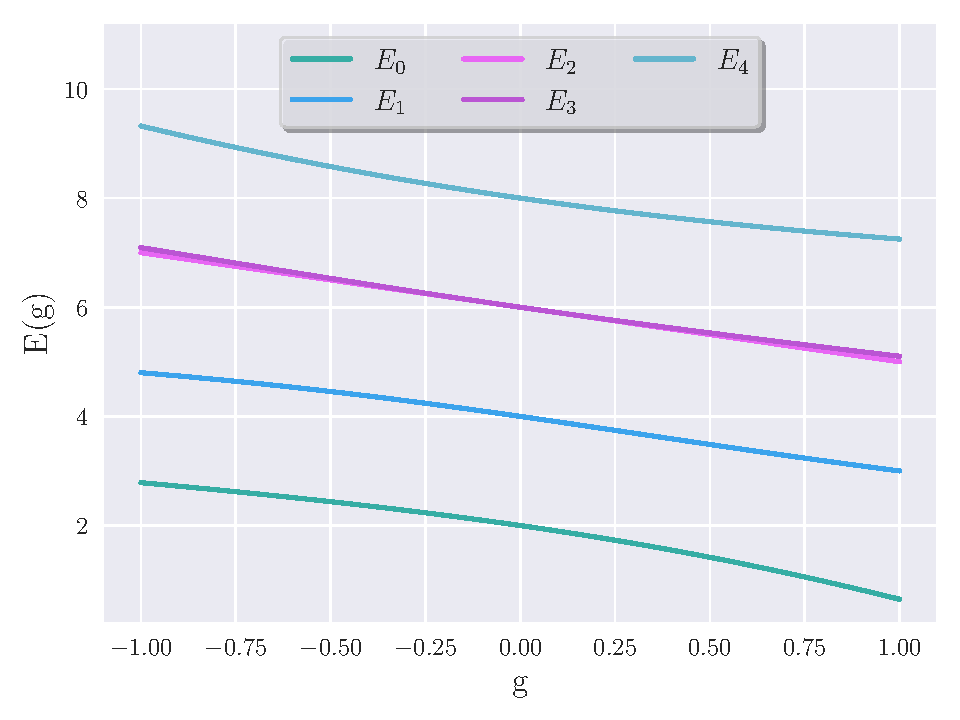
\includegraphics[width=\linewidth]{figs/CID.pdf}
        \end{subfigure}
        \hfill
        \begin{subfigure}{.49\textwidth}
            \centering
            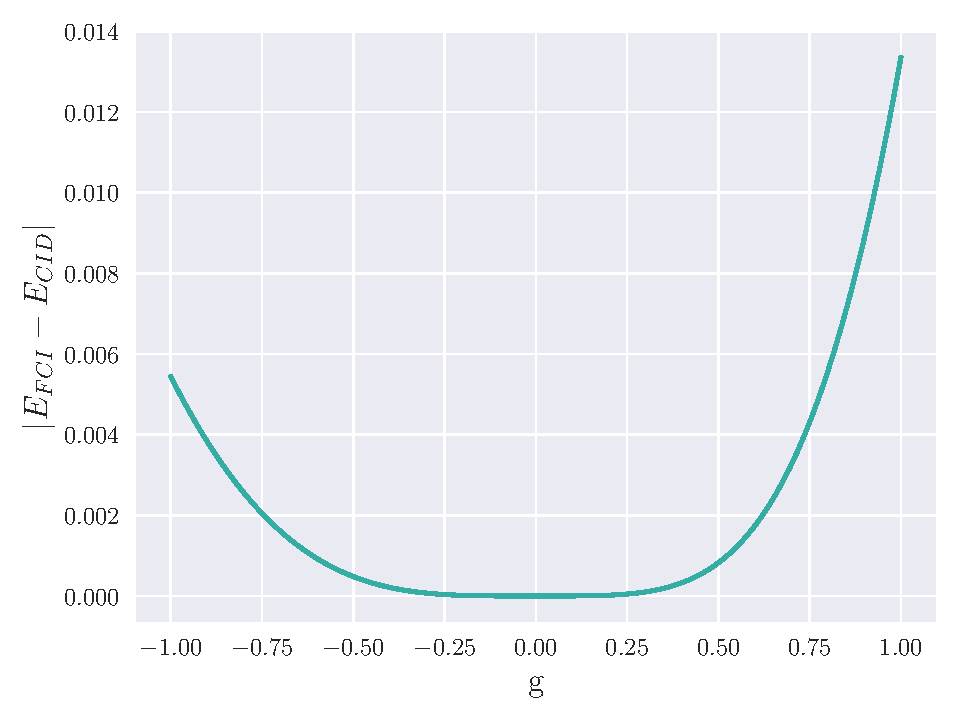
\includegraphics[width=\linewidth]{figs/FCI_CID_diff.pdf}
        \end{subfigure}
    \end{figure}
\end{frame}


\subsection{CI}
\begin{frame}
    \textcolor{Green}{\importanttext{Pros:}}
    \begin{itemize}
        \item Understandable and relatively easy to set up 
        \item Excited states thrown into the bargain
        \item Reduces the problem of FCI
        \item When adding contributions, we approach the exact energy (FCI).
    \end{itemize}
    \vspace{20px}
    \textcolor{Red}{\importanttext{Cons:}}
    \begin{itemize}
        \item Still quite computationally expensive
        \item Bad scaling for higher contributions
        \item What contributions to include might not be obvious
        \item Not size extensive 
    \end{itemize}
\end{frame}

\begin{frame}
    \frametitle{Hartree-Fock (HF)}
    Hartree-Fock methods approximate two body interactions as a mean field potential. This can be done by performing a unitary transformation on the orthonormal basis set $\mathset{\ket{\alpha}}$. The ground state ansatz energy is:
    \begin{align*}
        \inner{\Phi_0}{\hat{H}}{\Phi_0} = \sum_{\alpha=1}^N \inner{\alpha}{\hat{h}_0}{\alpha} + \frac{1}{2} \sum_{\alpha\beta=1}^N \innerAS{\alpha\beta}{\hat{v}}{\alpha\beta} 
    \end{align*}
    We aim to express this in a new (Hartree-Fock) basis $\mathset{\ket{i}}$.
    \begin{align*}
        \inner{\hatreefock{\Phi}_0}{\hat{H}}{\hatreefock{\Phi}_0} = \sum_{i=1}^{N} \inner{i}{\hat{h}_0}{i} + \frac{1}{2}\sum_{ij=1}^{N} \innerAS{ij}{\hat{v}}{ij}
    \end{align*}
    Of course we do not know this new basis a priori, but they are related by a unitary transformation $U$ where $U^\dagger = U^{-1}$. 
    \begin{align*}
        \ket{i} = U\ket{\alpha} = \sum_{\alpha} C_{i\alpha} \ket{\alpha}
    \end{align*}
    Since we have a unitary transformation, together with $\mathset{\ket{\alpha}}$ being orthonormal, the transformed basis $\mathset{\ket{i}}$ should also be orthonormal. 
\end{frame}

\subsection{HF}
\begin{frame}
    The new SP states must obey.
    \begin{align*}
        \sum_{ij=1}^{N} \braket{i|j} - \delta_{ij} = 0
    \end{align*}
    We formulate this as a minimization problem of the Hartree-Fock energy   
    \begin{align*}
        \inner{\hatreefock{\Phi}_0}{\hat{H}}{\hatreefock{\Phi}_0} = E[\hatreefock{\Phi}] = \sum_{i=1}^N \sum_{\alpha\beta=1}^n C^*_{i\alpha}C_{i\beta}\inner{\alpha}{\hat{h}_0}{\beta} + \frac{1}{2}\sum_{ij=1}^N \sum_{\alpha\beta\gamma\delta=1}^n C^*_{i\alpha} C^*_{j\beta} C_{i\gamma} C_{i\delta} \innerAS{\alpha\beta}{\hat{v}}{\delta\gamma} 
    \end{align*}
    With the constraint 
    \begin{align*}
        G = \sum_{ij=1}^N  \epsilon_{ij}\left( \sum_{\alpha\beta=1}^n C^*_{i\alpha}C_{j\beta} \braket{\alpha|\beta} - \delta_{ij}\right) = 0
    \end{align*}
    Then by taking the derivative w.r.t. the coefficients $C^*_{i\alpha}$ (minimizing w.r.t. $C$ or $C^*$ is arbitrary).
    \begin{align*}
        L[\hatreefock{\Phi}] &= E[\hatreefock{\Phi}] - G
    \end{align*}
    On obtains the eigenvalue problem (assuming we chose $\mathset{\ket{\alpha}}$ to be eigenstates of $\hat{h}_0$)
    \begin{align*}
        \sum_{\beta=1}^n \hatreefock{h}_{\alpha\beta} C_{i\beta} = \epsilon_i C_{i\alpha},\hspace{20px}
        \hatreefock{h}_{\alpha\beta} = \epsilon_\alpha \delta_{\alpha\beta} + \sum_{j=1}^{N} \sum_{\gamma\delta=1}^n C_{j\gamma}^* C_{j\delta} \innerAS{\alpha\gamma}{\hat{v}}{\beta\delta}
    \end{align*}
    This is often solved iteratively, until a stopping criterion is reached.
\end{frame}

\subsection{HF}
\begin{frame}
    Taking note of the interaction piece of $\hatreefock{h}_{\alpha\beta}$, this is nothing more than
    \begin{align*}
        \sum_{j=1}^{N} \sum_{\gamma\delta=1}^n C_{j\gamma}^* C_{j\delta} \innerAS{\alpha\gamma}{\hat{v}}{\beta\delta} = \sum_{j=1}^N \innerAS{\alpha j}{\hat{v}}{\beta j} = \sum_{j=1}^N \inner{\alpha j}{\hat{v}}{\beta j} - \inner{\alpha j}{\hat{v}}{j \beta} 
    \end{align*}
    often called the direct and exchange terms. The different states are affected by a mean field set up by all occupied states.
    \\[10pt]
    As an example, consider a basis set of three different hydrogen like s-orbitals, giving six total states when counting spin. Constructing Helium $(2e)$  and Beryllium $(4e)$ $ S= 0$ states, we can calculate the ground state energies and compare with CIS.

    \begin{table}[H]
        \centering
        \begin{tabular}{l|l|l|l|l|l}
        Atom      & $E_0$ & $E_{\text{CI}}$ & $\hatreefock{E_1}$ & $\hatreefock{E_c}$ & $E$ \\
        \hline
        Helium    & -2.7500     & -2.8385    & -2.8291 & -2.8311  & -2.9037    \\
        Beryllium & -13.7160     & -14.3621    & -14.4998 & -14.5083  &   -14.6674 
        \end{tabular}
        \caption{Showing the naive ground state energy expectation value $E_0$, the configuration interaction calculation $E_{\text{CI}}$, Hartree-Fock after 1 iteration and after convergence $\hatreefock{E_1}, \hatreefock{E_c}$ and the exact ground state energy using our Hamiltonian $E$.}
    \end{table}

\end{frame}

\subsection{HF}
\begin{frame}
    \textcolor{Green}{\importanttext{Pros:}}
    \begin{itemize}
        \item Computationally cheap
        \item Variational 
        \item Serves as a building block for other methods, changing to a HF basis can make another calculations simpler (i.e. perturbation theory)
    \end{itemize}
    \vspace{20px}
    \textcolor{Red}{\importanttext{Cons:}}
    \begin{itemize}
        \item If correlations are important, the mean field might not be a good approximation
        \item Possibility for not converging if the starting guess is not in a convex region around the minima
    \end{itemize}
\end{frame}

\begin{frame}
    \frametitle{Many body perturbation theory (MBPT)}
    Again, the exact ground state of the system is assumed to be an expansion of the ground state ansatz $\gs$ and excitations of this (1p1h, 2p2h...)
    \begin{align*}
        \ket{\Psi_0} = \gs + \sum_{m=1}^{\infty}C_m \ket{\Phi_m}
    \end{align*}
    With $m$ going over all $\gs$ excitations. There is no coefficient for $\gs$, since we have chosen intermediate normalization $\braket{\Phi_0 | \Psi_0} = 1$. $\ket{\Psi_0}$ is an eigenstate of the full Hamiltonian and we subtract the Schr\"{o}dinger equation from an arbitrary energy variable $\omega$. 
    \begin{align*}
        (\hat{H}_0 + \hat{V})\ket{\Psi_0} &= E \ket{\Psi_0} \\
        (\omega - \hat{H}_0)\ket{\Psi_0} &= (\omega-E+V)\ket{\Psi_0}
    \end{align*} 
    Defining two hermitian idempotent operators, for model space ($P$) and complimentary space ($Q$).
    \begin{align*}
        P = \ket{\Phi_0}\bra{\Phi_0}, \hspace{10px} Q = \sum_{m=1}^\infty \ket{\Phi_m}\bra{\Phi_m},\hspace{10px} P^2 = P, Q^2 = Q,\hspace{10px} [P,Q] = [\hat{H}_0, P] = [\hat{H}_0, Q] = 0
    \end{align*}
    Together they for the identity in the complete Hilbert space $P + Q = I$, which is useful since
    \begin{align*}
        \ket{\Psi_0} &= (P+Q)\ket{\Psi_0} = \gs + Q\ket{\Psi_0} \\
        Q\ket{\Psi_0} &= \ket{\Psi_0} - \gs 
    \end{align*}  
\end{frame}

\subsection{MBPT}
\begin{frame}
    When applying $Q$ from the left, the rewritten Schr\"{o}dinger equation becomes
    \begin{align*}
        Q\ket{\Psi_0} &= \hat{R}_0(\omega) (\omega - E + V)\ket{\Psi_0}, \hspace{20px} \hat{R}_0 (\omega) = \frac{Q}{\omega-\hat{H}_0} \\
        \ket{\Psi_0} &= \gs + \hat{R}_0(\omega) (\omega - E + V)\ket{\Psi_0}
    \end{align*}
    This is solved iteratively, often starting with the guess $\ket{\ord{\Psi_0}{0}} = \gs$. The final state $\ket{\Psi_0}$ can then be expressed as. 
    \begin{align*}
        \ket{\Psi_0} = \sum_{i=0}^\infty \left( \hat{R}_0(\omega) (\hat{V}-E+\omega) \right)^i \gs
    \end{align*}
    With an energy:
    \begin{align*}
        E = \inner{\Phi_0}{\hat{H}_0 + \hat{V}}{\Psi_0}= \ord{E}{0} + \Delta E = \ord{E}{0} +  \sum_{i=0}^\infty  \bra{\Phi_0} \hat{V}\left( \hat{R}_0(\omega) (\hat{V}-E+\omega) \right)^i \gs    
    \end{align*}
    Taking just the correlation energy $\Delta E$, we define the PT order by where we truncate this contribution
    \begin{align*}
        \Delta E = \sum_{i=0}^\infty \ord{\Delta E}{i},\hspace{20px} \ord{\Delta E}{i} = \bra{\Phi_0} \hat{V}\left( \hat{R}_0(\omega) (\hat{V}-E+\omega) \right)^i \gs
    \end{align*}
\end{frame}

\begin{frame}
    \frametitle{Different approaches, Rayleigh-Schr\"{o}dinger (RS)}
    Different choices of $\omega$ can now be made in order to obtain different types of PT expansions. 
    \\[10pt]
    Setting $\omega = E$ removes $E$ from $(\hat{V}-E+\omega)$, but it is still present in $\hat{R}_0(\omega = E)$, giving an implicit equation. This approach is called Brillouin-Wigner (BW) PT.
    \\[10pt] Setting $\omega = \ord{E}{0}$, we do not have the $E$ dependence problem for $\hat{R}_0$, and by setting $\Delta E = E - \ord{E}{0}$ we obtain.
    \begin{align*}
        \Delta E = \sum_{i=0}^\infty \ord{\Delta E}{i} = \sum_{i=0}^\infty \bra{\Phi_0} \hat{V}\left( \hat{R}_0(\omega) (\hat{V}-\Delta E) \right)^i \gs
    \end{align*}
    This does not seem to bring any improvement, since we still have an implicit equation. However, since $\hat{R}_0$ contains $Q$ and $\Delta E$ is just a scalar, $\hat{R}_0 \Delta E \ket{\Psi_0} = \Delta E \hat{R}_0 \ket{\Psi_0} = 0$, a pretty neat perturbative expansion can be formed when gathering terms of the same interaction order. 
\end{frame}

\subsection{RS}
\begin{frame}
    Explicitly, we expand $\Delta E$
    \begin{align*}
        \Delta E &= \inner{\Phi_0}{\hat{V}}{\Phi_0} + \inner{\Phi_0}{\hat{V}\hat{R}_0(\hat{V} - \Delta E)}{\Phi_0} + \inner{\Phi_0}{\hat{V}\hat{R}_0(\hat{V} - \Delta E)\hat{R}_0(\hat{V}-\Delta E)}{\Phi_0} + \ldots \\
        &=  \inner{\Phi_0}{\hat{V}}{\Phi_0} + \inner{\Phi_0}{\hat{V}\hat{R}_0\hat{V}}{\Phi_0} + \inner{\Phi_0}{\hat{V}\hat{R}_0(\hat{V} - \Delta E)\hat{R}_0\hat{V}}{\Phi_0} + \ldots \\
        &= \ord{E}{1} + \ord{E}{2} + \inner{\Phi_0}{\hat{V}\hat{R}_0\hat{V}\hat{R}_0\hat{V}}{\Phi_0} - \inner{\Phi_0}{\hat{V}\hat{R}_0\Delta E \hat{R}_0 \hat{V}}{\Phi_0} + \ldots
    \end{align*}
    And by inserting recursively for $\Delta E$, we get \textit{two} terms with three $\hat{V}$s, giving $\ord{E}{3}$. Higher orders of $\hat{V}$ will be given to $\ord{E}{4}, \ord{E}{5}, \ldots$.
    \begin{align*}
        &\inner{\Phi_0}{\hat{V}\hat{R}_0\hat{V}\hat{R}_0\hat{V}}{\Phi_0} - \inner{\Phi_0}{\hat{V}\hat{R}_0 (\ord{E}{1} + \ord{E}{2} + \ldots) \hat{R}_0 \hat{V}}{\Phi_0} + \ldots \\
        =&  \left( \inner{\Phi_0}{\hat{V}\hat{R}_0\hat{V}\hat{R}_0\hat{V}}{\Phi_0} - \ord{E}{1}\inner{\Phi_0}{\hat{V}\hat{R}_0^2 \hat{V}}{\Phi_0} \right) - \ord{E}{2}\inner{\Phi_0}{\hat{V}\hat{R}_0^2 \hat{V}}{\Phi_0} + \ldots \\
        =& \ord{E}{3} - \ord{E}{2}\inner{\Phi_0}{\hat{V}\hat{R}_0^2 \hat{V}}{\Phi_0} + \ldots
    \end{align*}
    We can now use this as a normal perturbative series that can be truncated at a specific interaction order (RS2, RS3 and so on). 
\end{frame}

\subsection{RS}
\begin{frame}
    In contrast to CI/Hartree-Fock, this is not a variational approach. There is no guarantee for convergence and results across different orders can vary.
    \\[10pt]
    If the SP energies are very close ($\hat{H}_0$), convergence might be a problem since the denominator of $\hat{R}_0$ can explode.
    \begin{align*}
        \ord{E}{2} = \inner{\Phi_0}{\hat{V}\hat{R}_0 \hat{V}}{\Phi_0} = \psum_m \inner{\Phi_0}{\hat{V}\frac{\ket{\Phi_m}\bra{\Phi_m}}{\ord{E}{0}-\hat{H}_0}\hat{V}}{\Phi_0}= \frac{1}{4} \sum_{ijab} \frac{|\inner{ij}{\hat{v}}{ab}|^2}{\epsilon_i + \epsilon_j - \epsilon_a - \epsilon_b}
    \end{align*}
    If the interaction is parametrized by a coupling constant, the coupling/SP energy ratio is crucial.
\end{frame}

\subsection{RS}
\begin{frame}
    \begin{figure}
        \begin{subfigure}{.49\textwidth}
            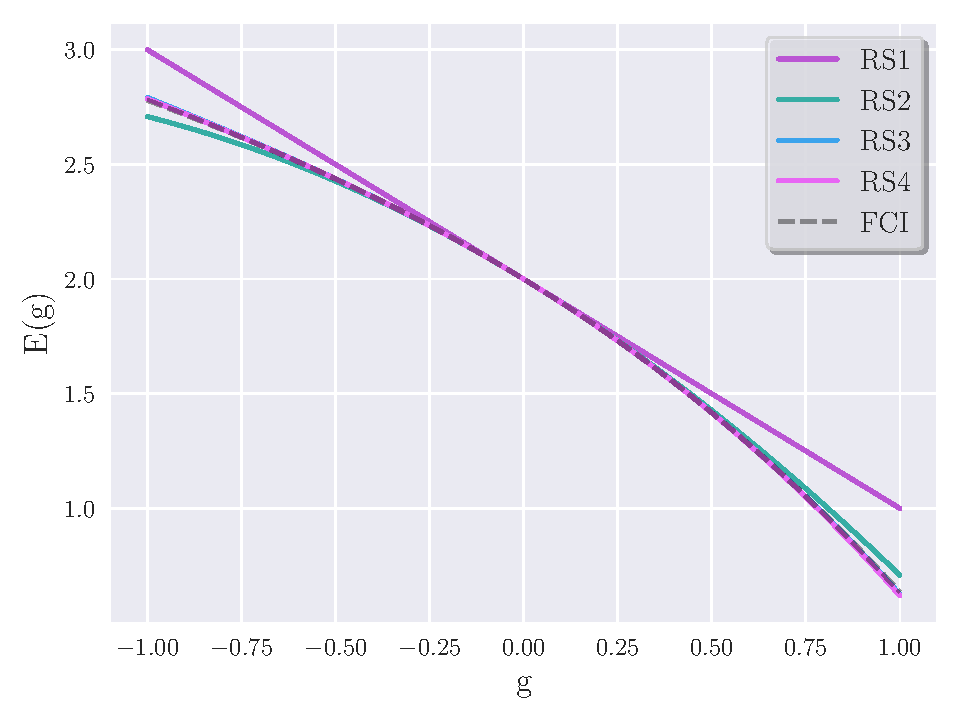
\includegraphics[width=\linewidth]{figs/RS_E.pdf}
        \end{subfigure}
        \hfill
        \begin{subfigure}{.49\textwidth}
            \centering
            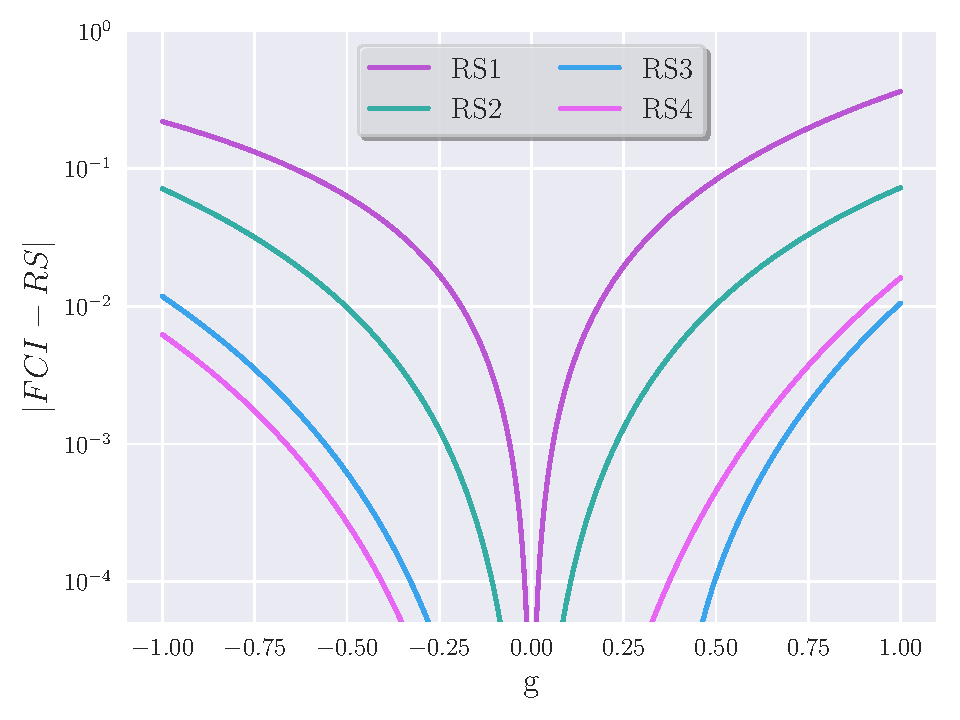
\includegraphics[width=\linewidth]{figs/RS_diff.pdf}
        \end{subfigure}
    \end{figure}
\end{frame}

\subsection{PT}
\begin{frame}
    \textcolor{Green}{\importanttext{Pros:}}
    \begin{itemize}
        \item Cheap compared with CI methods 
        \item Still capable of high accuracy
        \item Incorporate high order excitations, even at low order  
        \item Size extensive 
    \end{itemize}
    \vspace{20px}
    \textcolor{Red}{\importanttext{Cons:}}
    \begin{itemize}
        \item No guaranty for convergence
        \item Nonvariational, we have no energy bounds  
        \item Degeneracy (at least this formulation)
    \end{itemize}
\end{frame}

\end{document}